\monster{Antoleón}{4}{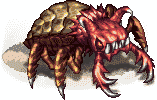
\includegraphics[width=0.26\textwidth]{./art/monsters/antlion.png}}
{
 PV: & \hfill 40 & PM: & \hfill 16\\
 FUE: & \hfill 3 & DEF: & \hfill 3 \\
 MAG: & \hfill 0 & RES: & \hfill 1 \\
 AGI: & \hfill 3 & Tamaño: & \hfill M\\
}
{
 \textbf{Mordida}: 2d de daño \hfill \textbf{Botín:} 300 Gil \\
 \textbf{Resistencia}:\earth \hfill \textbf{Inmune}:\blind 
 
 \mtech{Tormenta de Arena}{8}{1t}{3u}{Tú}{
 Todos los enemigos que se encuentren en el área de efecto deben hacer una tirada con DC 9. Si fallan, reciben 3d de daño de \hyperlink{type}{Tierra} y quedan \hyperlink{status}{Ciegos} por 3 turnos. }{\earth \blind} %\vspace{0.1cm} \hrule \vspace{0.1cm} 
 %\emph{"No ha problema. Los anteleones son bastante dóciles." -- Edward}
}
